\subsubsection{FACC}

\paragraph{Dendrograma de los clústeres obtenidos}

\begin{figure}[H]
    \centering
    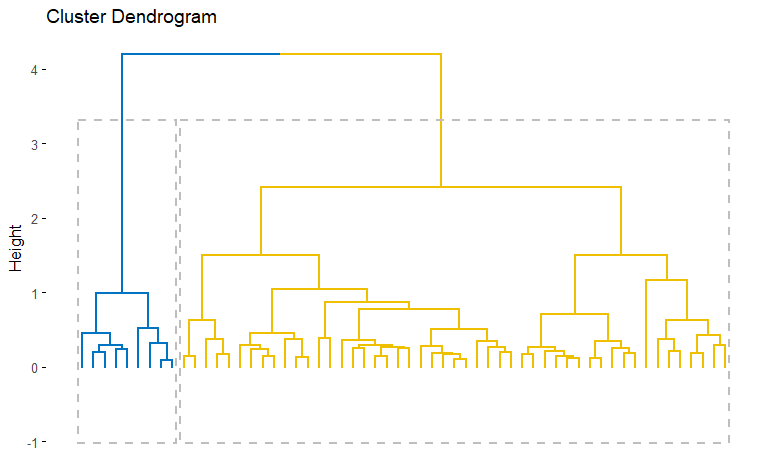
\includegraphics[scale = 0.8]{img/06-1-ccf.png}
    \caption{Dendograma }
    \label{fig:ccf_den}
\end{figure}

\paragraph{Distribución de los clústeres obtenidos en función de las dos primeras componentes principales}

\begin{figure}[H]
    \centering
    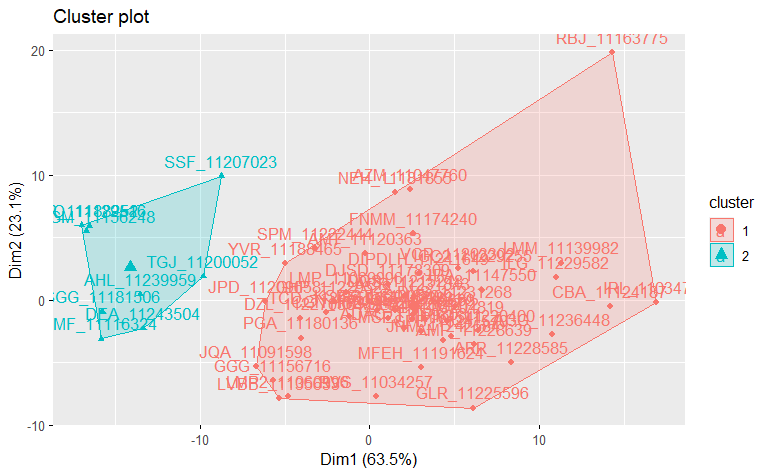
\includegraphics[scale = 0.8]{img/06-2-ccf.png}
    \caption{Cluster Plot}
    \label{fig:ccf_pc}
\end{figure}

\paragraph{Puntuación de Silhouette de los clústeres obtenidos}

\begin{figure}[H]
    \centering
    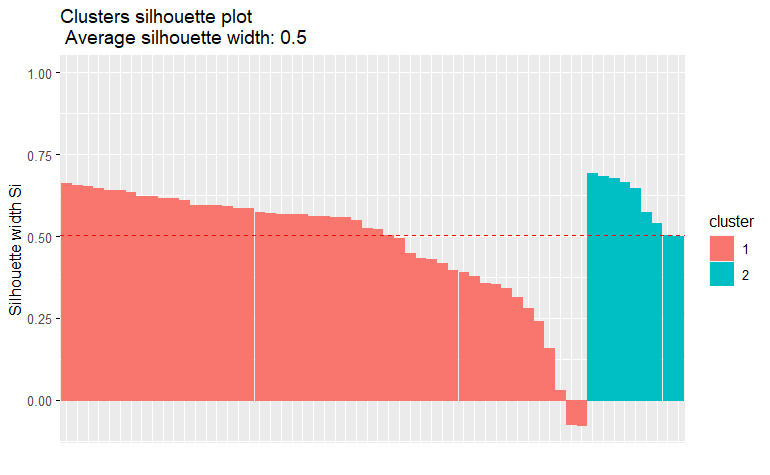
\includegraphics[scale = 0.8]{img/06-3-ccf.png}
    \caption{Silhouette Plot}
    \label{fig:ccf_si}
\end{figure}

\paragraph{Dendograma dividido en dos clústeres según los pacientes que han experimentado OAF}

\begin{figure}[H]
    \centering
    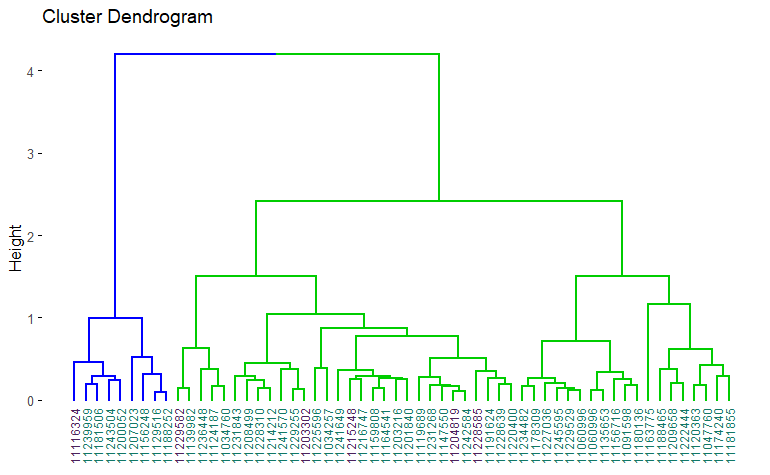
\includegraphics[scale = 0.8]{img/06-4-ccf.png}
    \caption{Dendograma Plot k = 2}
    \label{fig:ccf_ctg}
\end{figure}

\paragraph{Clasificación mediente Random Forest de los clústeres según las variables \textit{Cuantitativas} y \textit{Cualitativas} de la Tabla~\ref{tabla:variables_estudio_final}}

\begin{figure}[H]
    \centering
    \begin{lstlisting}[frame=single, basicstyle=\small\ttfamily]
        randomForest(formula = CLUSTER ~ ., data = newSMOTE_CCF) 
               Type of random forest: classification
                     Number of trees: 500
No. of variables tried at each split: 5

        OOB estimate of  error rate: 8.79%
Confusion matrix:
   1  2 class.error
1 46  3  0.06122449
2  5 37  0.11904762
    \end{lstlisting}
    \caption{Resultado de Random Forest utilizando variables \textit{Cuantitativas} y \textit{Cualitativas} de la Tabla~\ref{tabla:variables_estudio_final} y clasificación de clusters k = 2}\label{fig:random_forest_ccf_result_1}
\end{figure}

\paragraph{Mean Decrease Accuracy de las 5 primeras variables descriptivas utilizadas en Random Forest}

\begin{table}[H]
    \centering
    \begin{tabular}{lr}
        \toprule
        \textbf{Variable} & \textbf{Mean Decrease Accuracy} \\
        \midrule
        SCORE\_WOOD\_DOWNES\_INGRESO & 8.1087801 \\
        SCORE\_CRUCES\_INGRESO & 6.0526756 \\
        SAPI\_0\_8h & 3.9043532 \\
        TABACO & 3.2939905 \\
        ETIOLOGIA & 2.6061721 \\
        \bottomrule
    \end{tabular}
    \caption{Mean Decrease Accuracy}
\end{table}

\paragraph{Clasificación mediente Random Forest de los clústeres según Peridiograma utilizada para genear los mismos} 

\begin{figure}[H]
    \centering
    \begin{lstlisting}[frame=single, basicstyle=\small\ttfamily]
        randomForest(formula = CLUSTER ~ ., data = data_frame_merge_CCF) 
               Type of random forest: classification
                     Number of trees: 500
No. of variables tried at each split: 10

        OOB estimate of  error rate: 0%
Confusion matrix:
   1 2 class.error
1 49 0           0
2  0 9           0
    \end{lstlisting}
    \caption{Resultado de Random Forest utilizando FACC y clasificación de clusters k = 2}\label{fig:random_forest_ccf_result_RF_1}
\end{figure}

\paragraph{Distribución de la Importancia de FACC}

\begin{figure}[H]
    \centering
    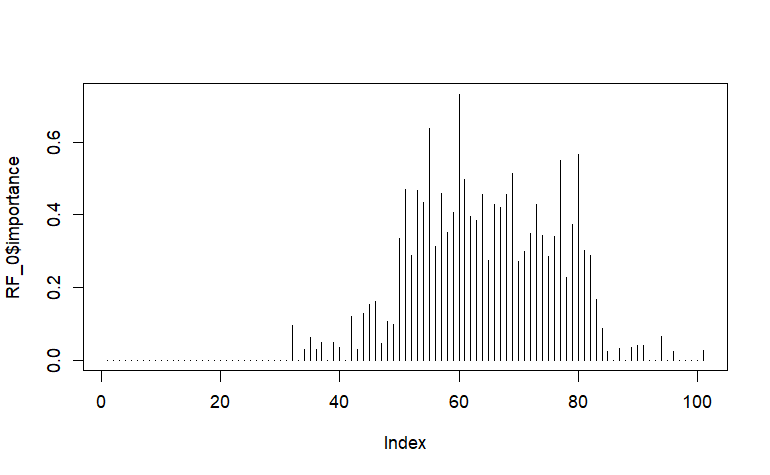
\includegraphics[scale = 0.8]{img/06-5-ccf.png}
    \caption{Dendograma Plot k = 2}
    \label{fig:ccf_imp}
\end{figure}

\paragraph{Media de los valores de Peridiograma en función de los clusters generados $k = 2$}

\begin{figure}[H]
    \centering
    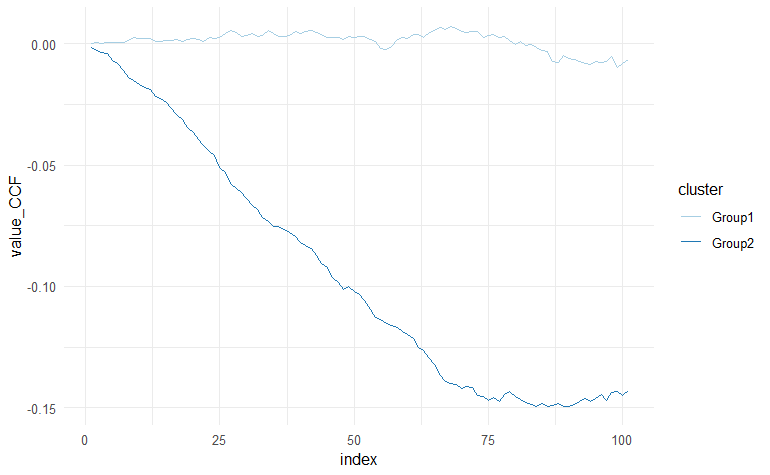
\includegraphics[scale = 0.8]{img/06-6-ccf.png}
    \caption{Dendograma Plot k = 2}
    \label{fig:ccf_cls}
\end{figure}